
\chapter{Introduction}

% TODO introduce heterogenous term
% \textit{Just imagine how you will get food without money because the credit card reader can't establish a connection to the bank.
% If you still got some cash you'll have to save it, since banks will not work anymore when the Web is gone. \textbf{(Really necessary?)}}

The Web is an ever growing institution, in all aspects that it covers.
Research on behalf of the Web attracts a great deal of attention, even more since modern life is already impossible without it.
% Imagine how you will get food without money because the credit card reader can't establish a connection to the bank.
% If you still got some cash you'll have to save it, since banks will not work anymore when the Web is gone.
The number of information and functionality providers for the Web is growing in the whole spectrum from bigger computing centers down to smaller devices.
Computing centers, growing in size and quantity, allow for massive amounts of data to be stored and accessed, but they also enable the construction and accessibility of more complex functionalities.
Ever smaller devices provide informations and functionalities to the Web, through their quickly increasing number.
Many of them are even providing access to the Web itself and thus leverage the effect of the growing Web.
For example mobile phones can act as a hotspot to grant Web access to others through \textrm{WiFi}.
All the smart \textrm{Things} with access to the Web start to form the \textrm{\gls{webofthings}}.
This can be every\textrm{Thing} from a temperature sensor to all electronic devices within a house.
These \textrm{Things} do not only provide sensor data but they can also be easily controlled through the Web.

Confronted with this rapid growth of the Web, an increasing number of human beings is exposed to it in their daily life and they get literally flooded with data and possibilities to govern them.
Even though they have access to all these services and data in the Web, they often lack the knowledge, necessary time or right approach to weave them together.
Users need ways to get appropriate informations, in the right moment, automatically and in a condensed matter that suits them best.
They have to be able to automate tedious tasks, e.g. detecting relevant changes in information resources and react on behalf of such changes.
\textit{\small{(More concrete example?)}}
This requires the identification of and filtering for user-specific information, appropriate timing, assembly and preprocessing of different information resources and finally the forwarding of outcomes to services in the web. 

Users don't want to be bound to specific services or applications, they want to use their preferred one, which they are used to and which helps them best to fulfill their needs.
Some of these services in the web offer ways to spread their data to other predefined services, but in very limited amount and parametrization.
Therefore users end up mashing informations or functionalities from different locations within the Web by hand.
This often means to execute similar tasks repeatedly by hand.
Moreover the completion of such a task suffers from latency due to the deferred detection of the initialization or because the user is just not able to execute the work at that time.
And also if the bits and pieces that form such a task could be separated, it is likely that some parts could be reused for other tasks or even by other people to get similar work done.

Since the data and the functionality already exists in the Web, the users could automate their work to some extent by orchestrating services and data.
Even though the access to services and data gets simpler, the average user is not able to fully exploit the Web.
Another challenge is that often a lot of effort needs to be invested, in understanding how the service works, before it can be fully exploited.
It is desirable to retain manageable mashing of services and data, while still exploiting their full potential.
There is a lot of research that goes towards an easy to orchestrate the Web, but they are either often complicated to wield themselves, mere data copy or static service compositions.

A big part of the informations, that become available to the users, are short-lived informations corresponding to certain state changes, and can therefore be modeled as events.
In this thesis we to introduce an event-driven conceptual model that enables the programmability of the Web and thus imposes reactivity on the Web.
We claim the whole Web as our information space, in which we listen for triggered events and in which we execute actions as a result.
Such an user-specific reactivity allows a personalization of the whole Web and a tool to govern its information flood.
This would allow users to orchestrate the Web in an intuitive way and to tailor reactivity to their needs.
Current orchestration approaches concentrate on data flow rather than on event flow, which are mere data copy/paste tasks than reactivity.
This makes us believe that an event-based conceptual model can overcome certain shortcomings of the existing solutions.


\begin{figure}[!ht]
  \centering
  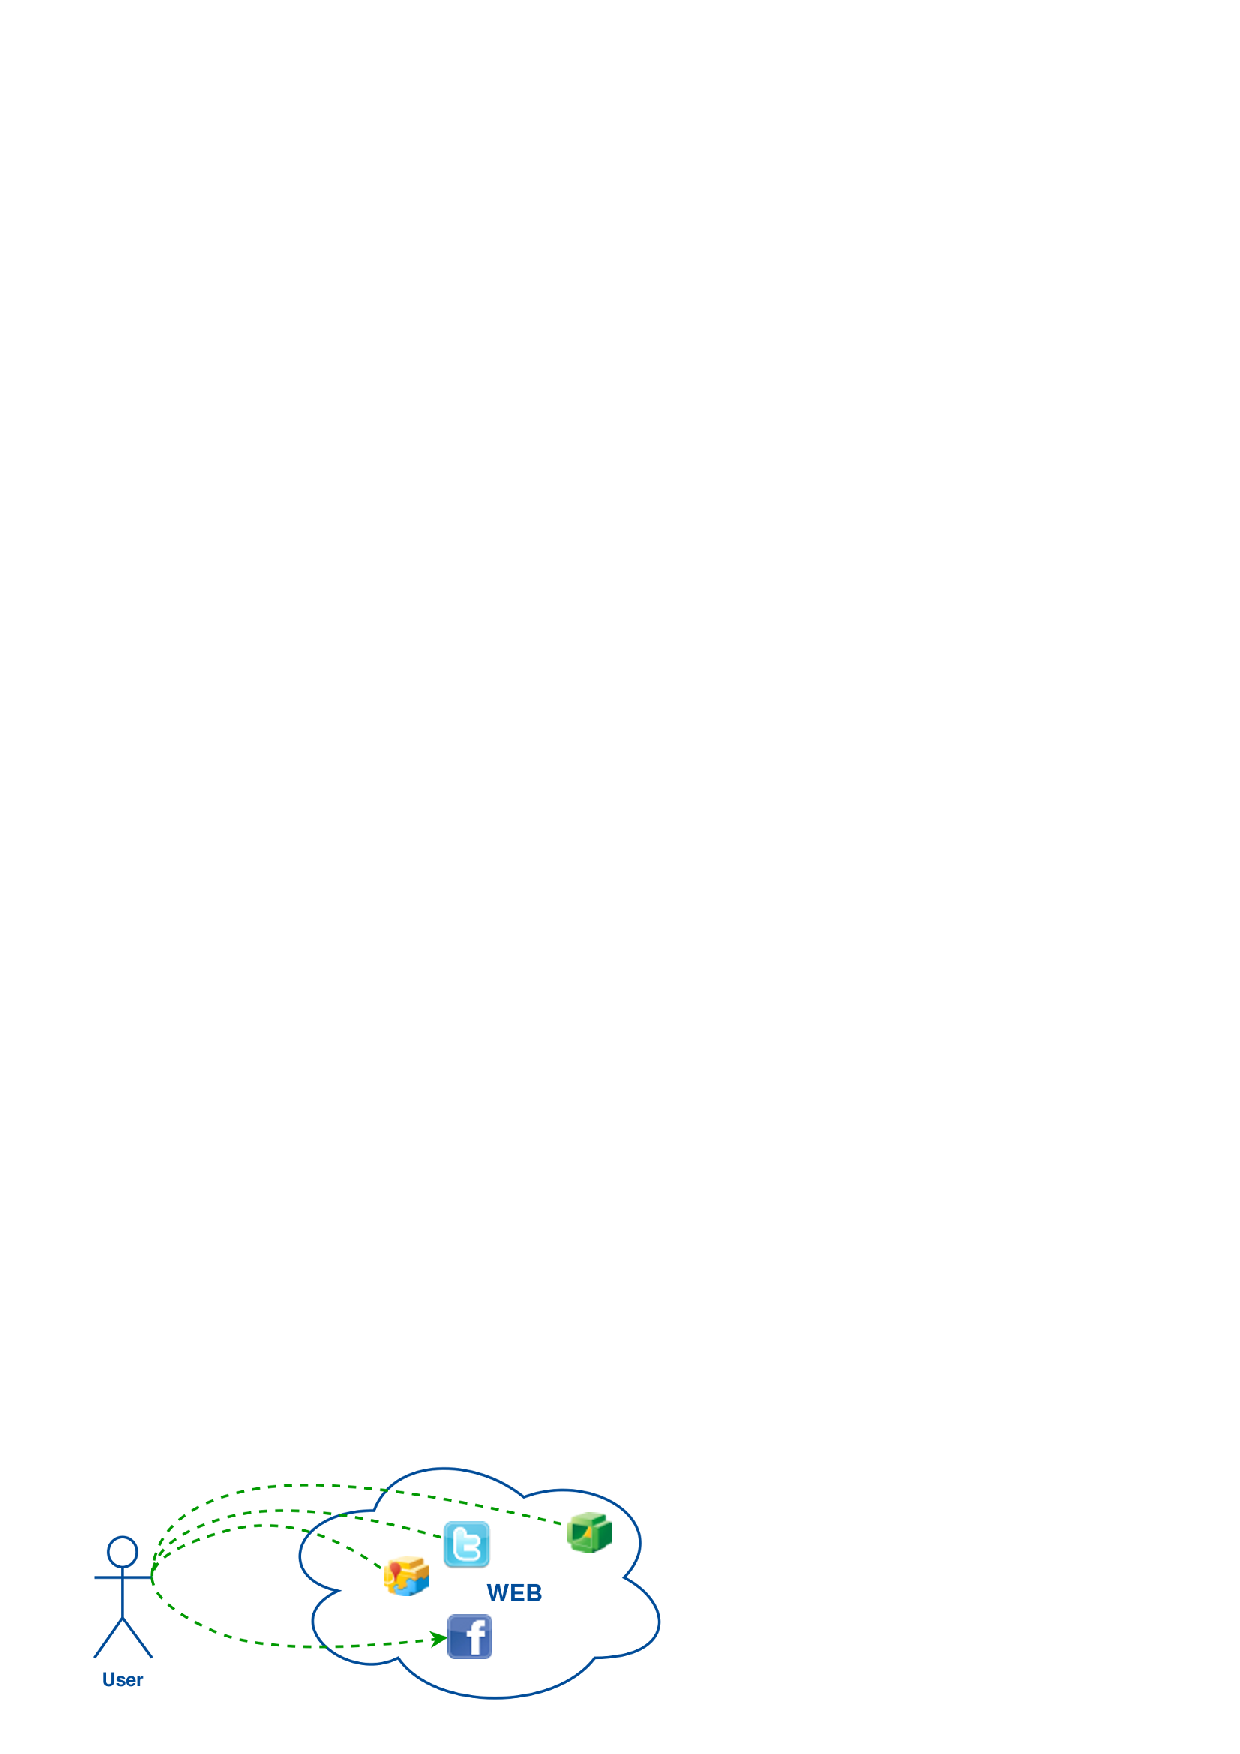
\includegraphics[width=0.7\textwidth]{figures/UsersWeildServicesInTheWeb}
  \caption{Users orchestrate the Web's Data and Functionality}
  \label{fig:UsersWeildServicesInTheWeb}
\end{figure}
% \textit{\small{MAKE NEW ONE! Figure with user orchestrating Web Resources}}
% \textit{\small{ewwww ugly figure....\\
% TODO show more concrete example with aha effect, light bulb. maybe parallel or serial events that turn into a result}}


% \textit{\small{TODO: use the word task or workflow?}}